\documentclass[a4paper,9pt]{scrartcl}
\usepackage{amssymb, amsmath}
\usepackage[margin=2.5cm]{geometry}
\usepackage[hyperfootnotes=false, pdfborder={0 0 0}, colorlinks=false]{hyperref}
\usepackage{color}
\usepackage{framed}
\usepackage{enumerate}
\usepackage{csquotes} 
\usepackage{listings}
\usepackage{graphicx}
\usepackage{float}
\usepackage{subcaption}

\definecolor{dkgreen}{rgb}{0,0.6,0}
\definecolor{gray}{rgb}{0.5,0.5,0.5}
\definecolor{mauve}{rgb}{0.58,0,0.82}


\setlength{\parskip}{0.4em}
\setlength{\parindent}{3em} 

\makeatletter
\renewcommand{\subsection}{\@startsection{subsection}{2}{0mm}
  {0.25\baselineskip} 
  {0.25\baselineskip} 
  {\normalfont\normalsize\bfseries}}
\makeatother

\makeatletter
\renewcommand{\section}{\@startsection{section}{1}{0mm}
  {1.5\baselineskip}
  {1\baselineskip} 
  {\normalfont\Large\bfseries}}
\makeatother






\newcommand\titletext{"Reinforcement Learning Assignment: FrozenLake"\\ 
\textit{Agents, Multi-Agent Systems and Reinforcement Learning} \\[0.5em] 
\textit{MSc, Artificial Intelligence, 2025}}
\title{\titletext}
\author{Michael Rice}
\usepackage{microtype}

\begin{document}

\maketitle

\section{Introduction}
This report will discuss the results from the second assignment of the CT5134 module. This assignment tackles Reinforcement Learning (RL) via the 
Q-Learning algorithm on the Frozen Lake toy problem, part of the famous 'Grid World' category of problems. Each of the results below are averaged
over a ten run window. 

\section{Hyperparameter Set 1 - Alpha(0.5), Gamma(0.9), Epsilon(0.1)}

The first set of hyperparameters to test were provided in the assignment and are as stated above. This test can be viewed as being designed to be 
a baseline from which to compare performance to later in the assignment. Below are three figures, each representing a different metric of the 
system's performance/learning. 

Firstly, the leftmost graph below represents the algorithm's reward earned per episode. This can be helpful in understanding the algorithms iterative
improvements over the episodes. As is evident here, the system approaches convergence relatively quickly, then proceeds to oscillate around
the level of convergence for the rest of the episodes. 

Secondly, the plot in the center shows the epsilon value over the length of the experiment. This value is kept constant here but will be varied,
and therefore rendering this plot more relevant, further into these experiments. 

Finally, the rightmost graph depicts the percentage of episodes, averaged again, that reach the 'Win' state. Again, as in the first graph, this
plot shows early convergence followed by stagnation, reaching a peak win rate of just over \textbf{91\%}.

\begin{figure}[H]
\centering
\begin{subfigure}[b]{0.32\textwidth}
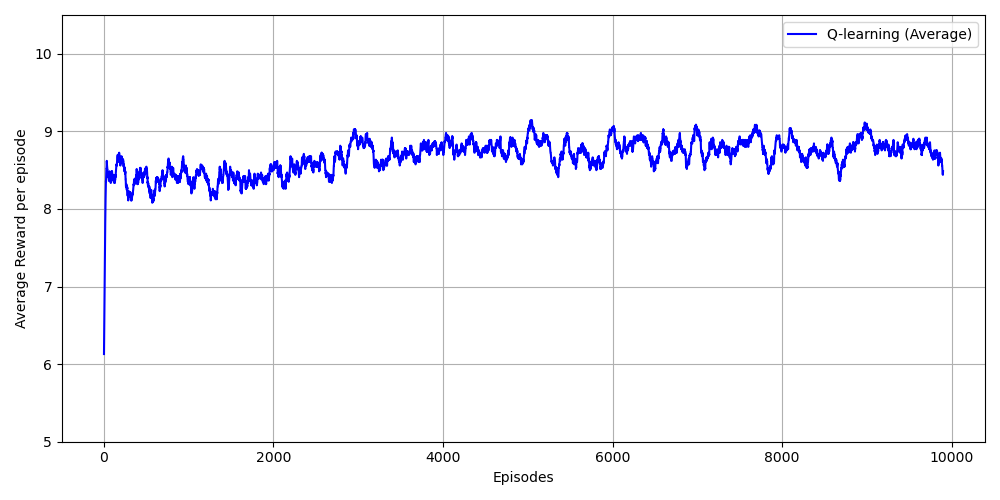
\includegraphics[width=\textwidth]{images/q_learning_rewards_avg(1).png}
\caption{Run Averaged Reward Per Episode}
\label{fig:set1_rewards}
\end{subfigure}
\hfill
\begin{subfigure}[b]{0.32\textwidth}
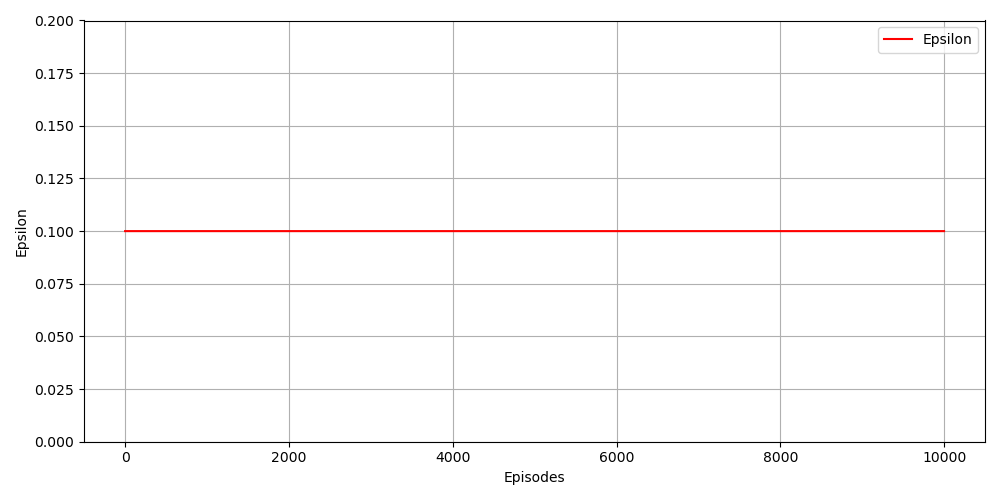
\includegraphics[width=\textwidth]{images/q_learning_epsilon_avg(1).png}
\caption{Run Averaged Epsilon}
\label{fig:set1_epsilon}
\end{subfigure}
\hfill
\begin{subfigure}[b]{0.32\textwidth}
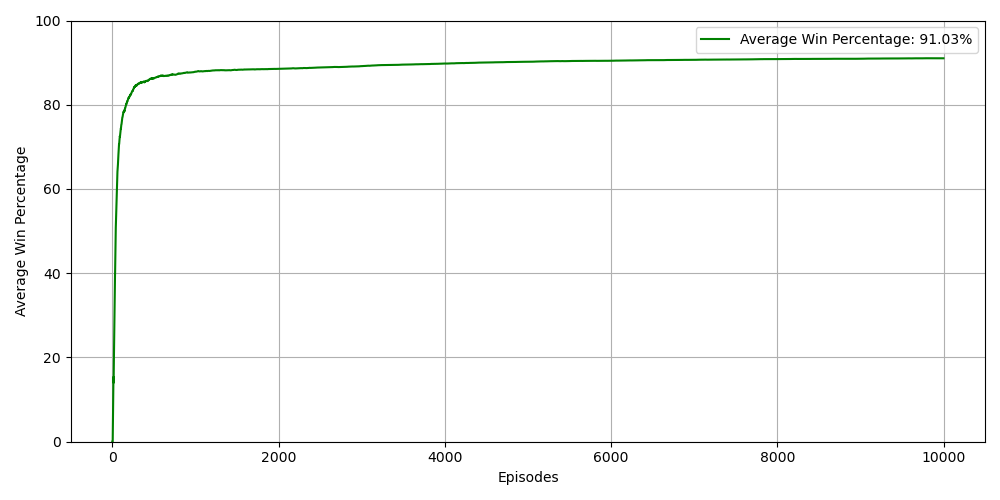
\includegraphics[width=\textwidth]{images/q_learning_win_percentage_avg(1).png}
\caption{Run Averaged Win \%}
\label{fig:set1_winpercent}
\end{subfigure}
\caption{Metrics for Hyperparameter Set 1}
\label{fig:set1_metrics}
\end{figure}

The figure below shows the Q-value results from this first foray into the Frozen Lake problem. As can be seen, each of the predefined 
'hole' states, as well as the 'win' state, end the process with a Q-value of 0, as they are terminal states. Other states that are hole adjacent 
tend to end with negative Q-values due to the fact that they do not explicitly provide a worse reward by moving to that state, but choosing to move to them 
negatively effects overall episodic reward but placing us in proximity to such negative termini. Remaining states increase in value the further right and 
down they are, as this means they are closer to the goal state, and thus a substantial reward. There are also other notable artifacts that occur due to 
the structure of this problem, such as the fact that non-terminal states are more likely to have a higher reward if they are above the diagonal than below.
This is likely a result of the placement of the hole states, meaning being below the diagonal is generally less likely to result in an optimal path.  


\begin{figure}[H]
\centering
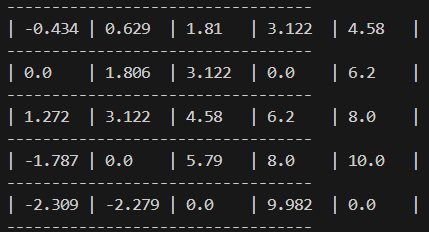
\includegraphics[width=0.4\textwidth]{images/qvalues(1).png}
\caption{Action Value Estimates for Each State}
\label{fig:set1_qvalues}
\end{figure}

\section{Same Hyperparameter Set w/ Epsilon Decay - Linear, Quadratic and Cubic}

In this portion of the experiment, the starting hyperparameters remained the exact same as the section previous. However, this time
throughout each run, the epsilon value would be decayed in order to alter the exploration/exploitation balance to aid in the discovery of
an optimal path through the grid.

Three different methods of epsilon decay were tried during this section of the experiment; Linear, Quadratic and Cubic, each starting at a 
value of 0.1 as before, and ending each run at 0. As can be seen in the plots below, the Linear method retains a constant level of decay
throughout each run, while both the Quadratic and Cubic methods keep larger values of epsilon for longer. This means both of these 
non-linear methods are more explorative at the beginning of the runs, with a faster decay at the end (exploitation).

\begin{figure}[H]
\centering
\begin{subfigure}[b]{0.32\textwidth}
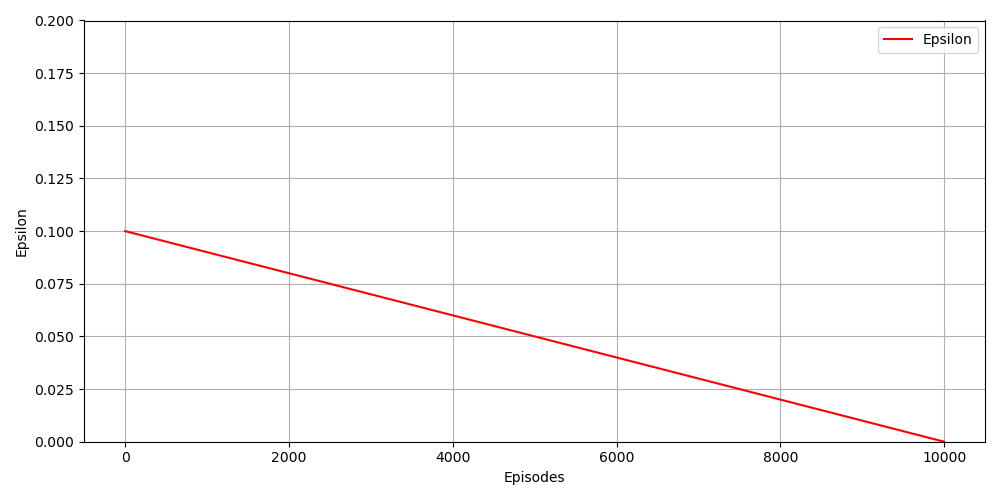
\includegraphics[width=\textwidth]{images/q_learning_epsilon_avg(2)(0).png}
\caption{Linear Decay}
\label{fig:decay_linear}
\end{subfigure}
\hfill
\begin{subfigure}[b]{0.32\textwidth}
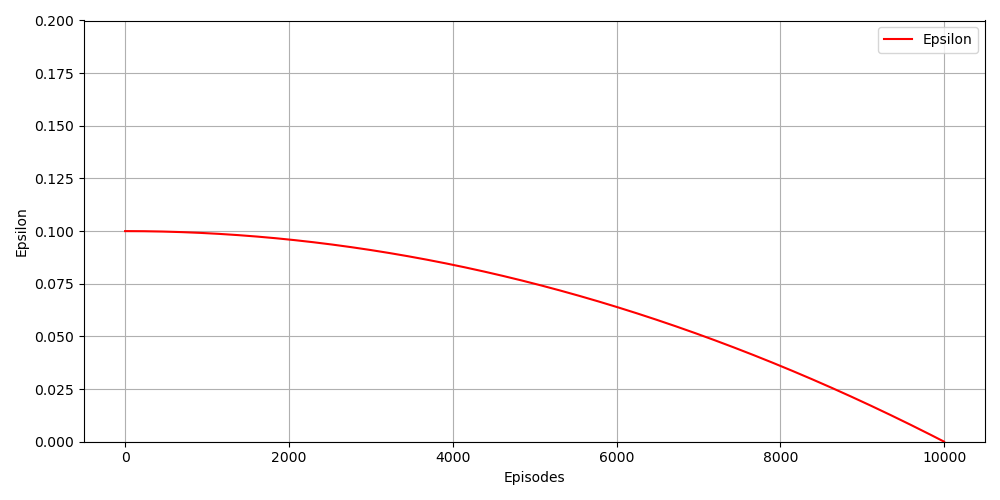
\includegraphics[width=\textwidth]{images/q_learning_epsilon_avg(2)(1).png}
\caption{Quadratic Decay}
\label{fig:decay_quadratic}
\end{subfigure}
\hfill
\begin{subfigure}[b]{0.32\textwidth}
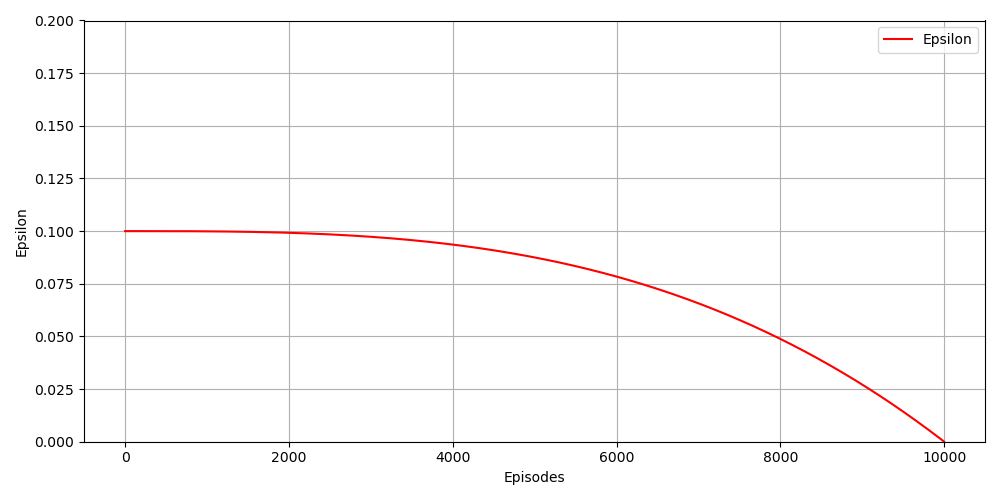
\includegraphics[width=\textwidth]{images/q_learning_epsilon_avg(2)(2).png}
\caption{Cubic Decay}
\label{fig:decay_cubic}
\end{subfigure}
\caption{Epsilon Decay Schedules}
\label{fig:decay_schedules}
\end{figure}

The best performing method of epsilon decay was Linear, perhaps indicating that this problem favored a less explorative approach, as linear was the least
explorative method tested. The reward per episode and win percentage graphs are shown below, with a clear improvement in the trend of the reward per episode, 
in comparison to the initial test. The final win percentage was also improved from the first test, to \textbf{95.24\%}, a gain of over 4\%.

\begin{figure}[H]
\centering
\begin{subfigure}[b]{0.45\textwidth}
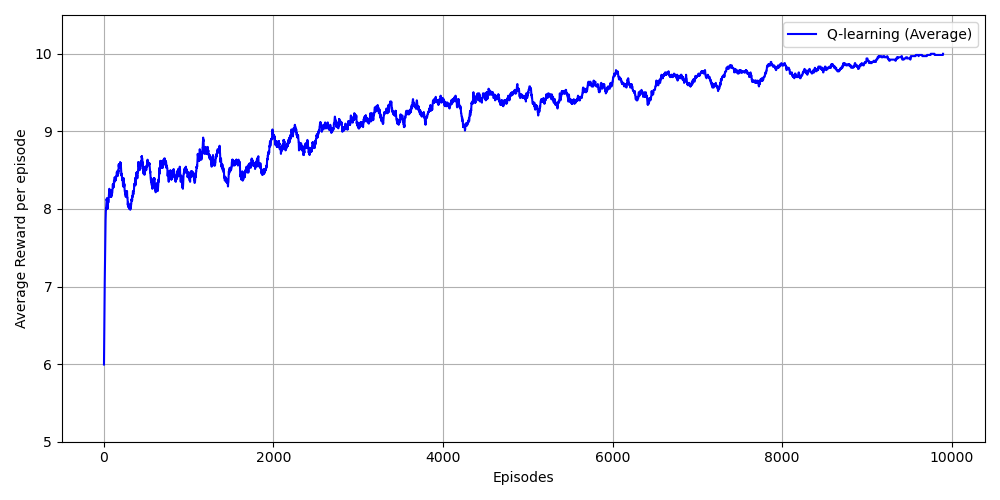
\includegraphics[width=\textwidth]{images/q_learning_rewards_avg(2)(0).png}
\caption{Reward Per Episode}
\label{fig:decay_rewards}
\end{subfigure}
\hfill
\begin{subfigure}[b]{0.45\textwidth}
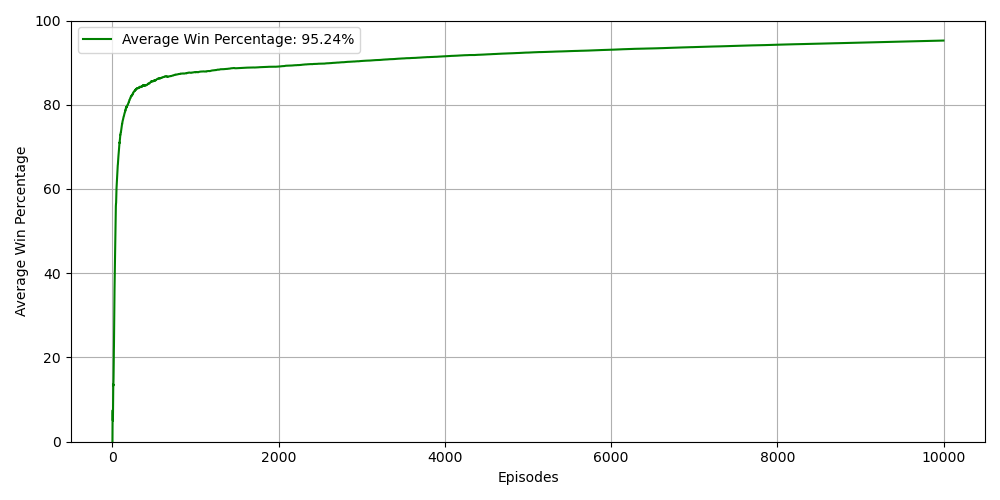
\includegraphics[width=\textwidth]{images/q_learning_win_percentage_avg(2)(0).png}
\caption{Win Percentage}
\label{fig:decay_winpercent}
\end{subfigure}
\caption{Performance with Linear Decay}
\label{fig:decay_performance}
\end{figure}

Finally, for this section, the Q-Values exhibit most of the same characteristics as the Q-Values in the initial experiment, with one major notable
change. As mentioned in the first section, the Q-Values above the diagonal tended to be higher than those below due to the presence of more 'hole' 
states below the diagonal. However, due to the increased exploitation by the linear epsilon delay versus a constant epsilon in this attempt, positive
values appear to be more even, aside from the obvious exception of the bottom left of the state space, which is a trap when it comes to 
improving episodic rewards.


\begin{figure}[H]
\centering
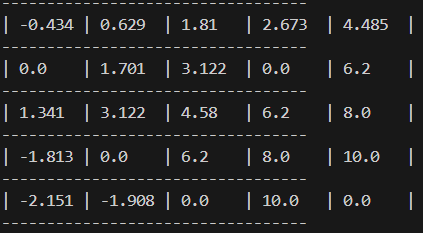
\includegraphics[width=0.4\textwidth]{images/qvalues(2)(0).png}
\caption{Action Value Estimates}
\label{fig:set2_qvalues}
\end{figure}

\section{Hyperparameter Set 3 - Alpha(0.7), Gamma(0.95), Epsilon(0.001)}

Finally, using the learnings taken from the previous experiments, a new set of hyperparameters were to be designed. As previously mentioned,
these previous tests pointed to increased exploitation improving the algorithm's performance, therefore this was the chosen direction when
selecting these hyperparameters. After a number of tests, values of Alpha=0.7, Gamma=0.95 and Epsilon=0.001. This approach maximised exploitation,
with little to no randomness/exploration.

As is evident in the reward per episode and win percentage plots below, the algorithm converges towards the optimal solution much quicker with these
parameters. Furthermore, the overall percentage of episodes in which the win state was reached was again improved, reaching \textbf{99.79\%},
another sizeable improvement of over 4\%.

\begin{figure}[H]
\centering
\begin{subfigure}[b]{0.32\textwidth}
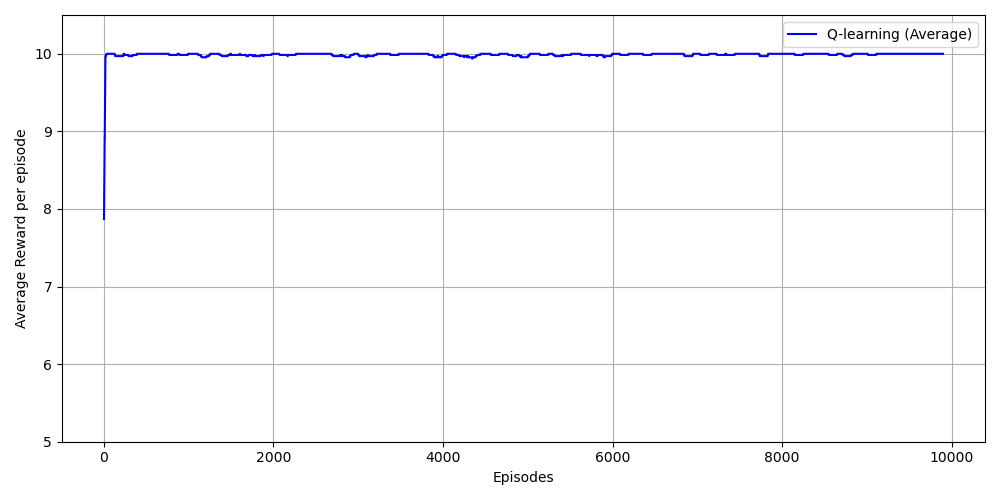
\includegraphics[width=\textwidth]{images/q_learning_rewards_avg(3).png}
\caption{Run Averaged Reward}
\label{fig:set3_rewards}
\end{subfigure}
\hfill
\begin{subfigure}[b]{0.32\textwidth}
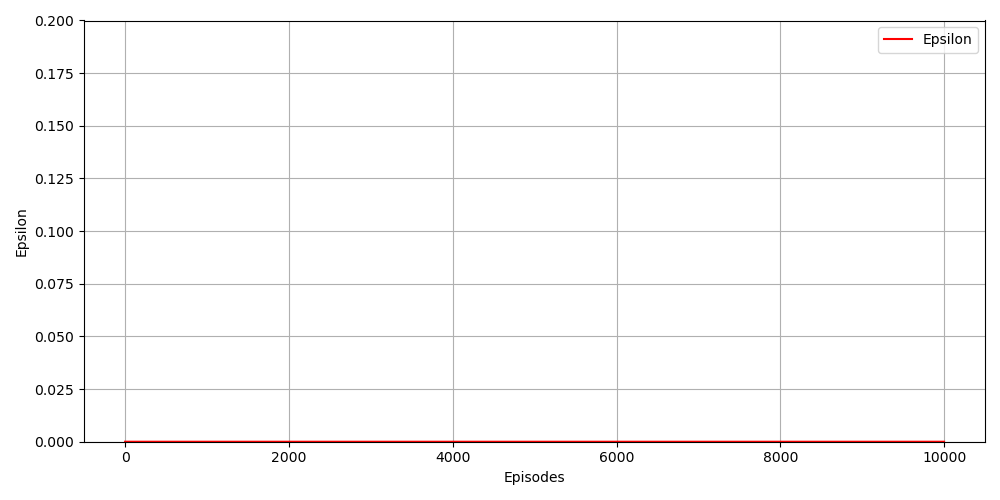
\includegraphics[width=\textwidth]{images/q_learning_epsilon_avg(3).png}
\caption{Epsilon Decay}
\label{fig:set3_epsilon}
\end{subfigure}
\hfill
\begin{subfigure}[b]{0.32\textwidth}
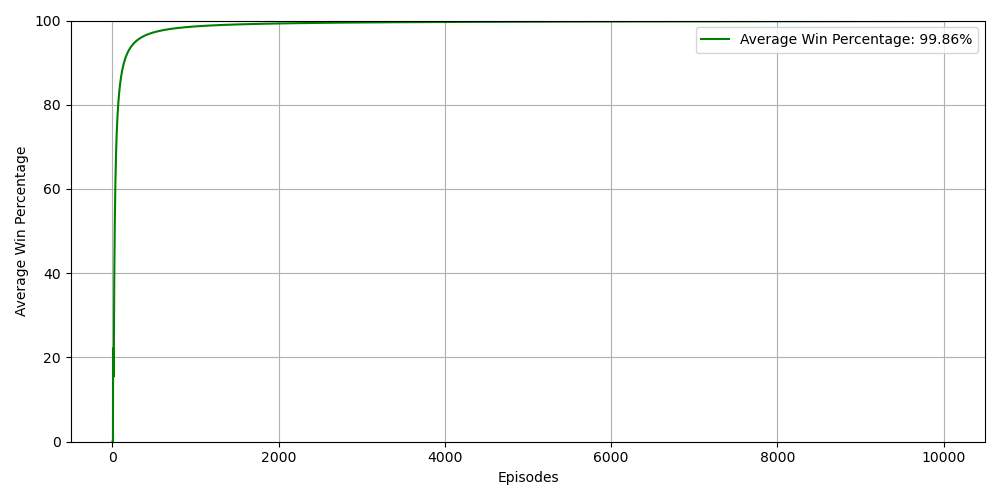
\includegraphics[width=\textwidth]{images/q_learning_win_percentage_avg(3).png}
\caption{Win Percentage}
\label{fig:set3_winpercent}
\end{subfigure}
\caption{Metrics for Custom Hyperparameters}
\label{fig:set3_metrics}
\end{figure}

When comparing the eventual Q-Values for these hyperparameters to the previous two experiments, it is evident that several changes took place.
Firstly, these parameters punish the bottom left corner of the state space even more heavily than before, this time including the (2,0) state,
which held a positive value for both previous sets of arguments. Secondly, the top right corner of the state space is now also actively 
discouraged, without having any hole states, which had not occurred previously. This shows that the algorithm is learning to choose the quickest 
possible path through the world, considering both hole states and overall step count. The hole state of (1,3) is likely responsible for this,
as having to go around it increases overall step count, thus lowering reward, which leads to the states which would be involved in travelling 
around this hole state to be discouraged. Finally, the chosen path is much more evident in this section, with the algorithm clearly favouring
repetitions of the (Right,Down) action pair until the goal state is reached. This is the reason why state (4,3) has a lower value than (3,4),
despite both being win state adjacent. As a final note, none of the epsilon decline methods had any major effect on the result of this 
experiment, meaning any of them, or none, could be used.


\begin{figure}[H]
\centering
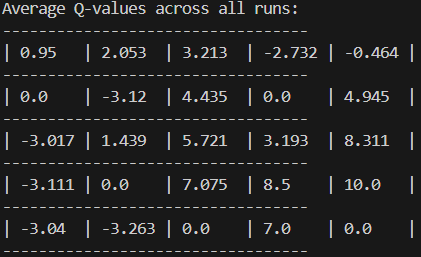
\includegraphics[width=0.4\textwidth]{images/qvalues(3).png}
\caption{Action Value Estimates}
\label{fig:set3_qvalues}
\end{figure}

\end{document}
